\documentclass[a4paper,12pt]{article}[abntex2]
\bibliographystyle{abntex2-alf}
\usepackage{siunitx} % Fornece suporte para a tipografia de unidades do Sistema Internacional e formatação de números
\usepackage{booktabs} % Melhora a qualidade das tabelas
\usepackage{tabularx} % Permite tabelas com larguras de colunas ajustáveis
\usepackage{graphicx} % Suporte para inclusão de imagens
\usepackage{newtxtext} % Substitui a fonte padrão pela Times Roman
\usepackage{ragged2e} % Justificação de texto melhorada
\usepackage{setspace} % Controle do espaçamento entre linhas
\usepackage[a4paper, left=3.0cm, top=3.0cm, bottom=2.0cm, right=2.0cm]{geometry} % Personalização das margens do documento
\usepackage{lipsum} % Geração de texto dummy 'Lorem Ipsum'
\usepackage{fancyhdr} % Customização de cabeçalhos e rodapés
\usepackage{titlesec} % Personalização dos títulos de seções
\usepackage[portuguese]{babel} % Adaptação para o português (nomes e hifenização
\usepackage{hyperref} % Suporte a hiperlinks
\usepackage{indentfirst} % Indentação do primeiro parágrafo das seções
\sisetup{
  output-decimal-marker = {,},
  inter-unit-product = \ensuremath{{}\cdot{}},
  per-mode = symbol
}
\setlength{\headheight}{14.49998pt}

\DeclareSIUnit{\real}{R\$}
\newcommand{\real}[1]{R\$#1}
\usepackage{float} % Melhor controle sobre o posicionamento de figuras e tabelas
\usepackage{footnotehyper} % Notas de rodapé clicáveis em combinação com hyperref
\hypersetup{
    colorlinks=true,
    linkcolor=black,
    filecolor=magenta,      
    urlcolor=cyan,
    citecolor=black,        
    pdfborder={0 0 0},
}
\usepackage[normalem]{ulem} % Permite o uso de diferentes tipos de sublinhados sem alterar o \emph{}
\makeatletter
\def\@pdfborder{0 0 0} % Remove a borda dos links
\def\@pdfborderstyle{/S/U/W 1} % Estilo da borda dos links
\makeatother
\onehalfspacing

\begin{document}

\begin{titlepage}
    \centering
    \vspace*{1cm}
    \Large\textbf{INSPER – INSTITUTO DE ENSINO E PESQUISA}\\
    \Large ECONOMIA\\
    \vspace{1.5cm}
    \Large\textbf{Estudos do Case 3 - H.E.B}\\
    \vspace{1.5cm}
    Prof. Heleno Piazenini Vieira\\
    Prof. Auxiliar \\
    \vfill
    \normalsize
    Hicham Munir Tayfour, \href{mailto:hichamt@al.insper.edu.br}{hichamt@al.insper.edu.br}\\
    5º Período - Economia A\\
    \vfill
    São Paulo\\
    Outubro/2024
\end{titlepage}

\newpage
\tableofcontents
\thispagestyle{empty} % This command removes the page number from the table of contents page
\newpage
\setcounter{page}{1} % This command sets the page number to start from this page
\justify
\onehalfspacing

\pagestyle{fancy}
\fancyhf{}
\rhead{\thepage}


\section{\textbf{Relação do texto com o tema: "Primeira Guerra Mundial e o pós-guerra: as questões econômicas brasileiras."}}

A Primeira Guerra Mundial e o período pós-guerra tiveram impactos profundos na economia brasileira, com efeitos que se manifestaram tanto no curto prazo quanto nos anos subsequentes. A partir dos textos fornecidos, podemos observar como o Brasil, particularmente sua economia baseada na exportação de café, passou por um ciclo de desafios e ajustes, refletindo as dinâmicas internacionais e as peculiaridades da conjuntura nacional.

Durante a Primeira Guerra Mundial, o Brasil enfrentou uma série de dificuldades estruturais, exacerbadas pela dependência da exportação de café e pela interrupção dos fluxos comerciais globais. Um dos principais problemas abordados nos textos é o estrangulamento da capacidade de escoamento da safra de café devido à falta de navios, em grande parte causada pela neutralidade do Brasil no conflito e pela retenção de navios estrangeiros, especialmente alemães. Com a expropriação dos navios alemães, uma solução temporária foi encontrada, mas ainda assim havia limitações técnicas para sua imediata utilização. Essa dificuldade, somada ao aumento dos estoques de café no porto de Santos e à incapacidade do sistema bancário de financiar adequadamente o setor, criou um ambiente de crise interna.

O texto também destaca como, no cenário da guerra, o Brasil enfrentou pressões inflacionárias e sociais. A emissão de notas inconversíveis para financiar a safra de 1917 levou a um aumento generalizado dos preços, especialmente de alimentos, o que resultou na primeira grande onda de greves e manifestações operárias na história do país. Esse fenômeno refletia a transformação social das grandes cidades brasileiras, que, durante o período de guerra, vivenciaram mudanças estruturais, com o aumento da população urbana e a crescente organização da classe trabalhadora.

No pós-guerra, as questões econômicas brasileiras foram marcadas por um período inicial de boom seguido de uma recessão severa, entre 1919 e 1922. O boom econômico, que se seguiu ao armistício de 1918, foi impulsionado pelo aumento dos preços das commodities no mercado internacional, particularmente o café. A geada de 1918 em São Paulo, que reduziu significativamente a oferta global de café, combinada com a recuperação da demanda global reprimida durante o conflito, levou a uma explosão nas exportações brasileiras. O superávit comercial de 1919 reflete esse contexto, com o Brasil capitalizando o aumento dos preços e a maior demanda internacional.

Entretanto, o boom teve curta duração. A partir de meados de 1920, a adoção de políticas monetárias restritivas pelos principais centros financeiros internacionais (Estados Unidos e Reino Unido), em resposta à inflação pós-guerra, precipitou uma recessão global. Para o Brasil, essa mudança resultou na queda abrupta dos preços das commodities, incluindo o café, o que teve um efeito devastador sobre a economia nacional. A súbita queda das exportações coincidiu com um aumento tardio nas importações, criando uma pressão adicional sobre a balança comercial e levando à depreciação do mil-réis.

A crise cambial e a recessão global de 1920-1921 tiveram profundas consequências na condução da política econômica brasileira. O governo, preocupado com a rápida desvalorização cambial e suas repercussões fiscais e inflacionárias, adotou medidas para tentar estabilizar a situação. Uma das principais preocupações era o impacto da desvalorização sobre o orçamento federal, especialmente considerando que grande parte das receitas do governo dependia de tarifas alfandegárias e que havia um volume significativo de despesas em moeda estrangeira, particularmente após o grande programa de obras públicas iniciado pelo governo Epitácio Pessoa. O impacto inflacionário também era uma preocupação central, dado que a desvalorização cambial afetava diretamente os salários reais e a estrutura de custos no Brasil da Primeira República.

Além das questões fiscais e cambiais, o colapso dos preços internacionais do café representou uma ameaça direta à economia brasileira, levando o governo a buscar formas de intervenção no mercado. A criação da Carteira de Redesconto do Banco do Brasil, aprovada em outubro de 1920, foi uma tentativa de fornecer liquidez emergencial ao setor privado, permitindo que o banco redistribuísse crédito para sustentar o mercado de café. No entanto, essa foi uma solução provisória, e o governo foi forçado a intervir mais diretamente no início de 1921, autorizando o financiamento de compras de café com o auxílio de crédito externo, obtido em bancos britânicos.

O colapso cambial de 1920-1921, combinado com a crise no setor cafeeiro, revelou a vulnerabilidade do Brasil às flutuações dos mercados globais, especialmente no que diz respeito às commodities. O governo foi forçado a recorrer a medidas de austeridade fiscal para tentar conter o desequilíbrio orçamentário e controlar a inflação. A emissão de letras de curto prazo e o crescimento da dívida pública com o Banco do Brasil, por sua vez, criaram um círculo vicioso de aumento da base monetária e novas pressões inflacionárias. Apesar dos esforços de intervenção, a situação fiscal do governo continuou crítica ao longo de 1922, com o déficit orçamentário atingindo níveis alarmantes.

Dessa forma, os textos demonstram como a Primeira Guerra Mundial e o pós-guerra foram períodos de extrema volatilidade para a economia brasileira. O boom inicial das exportações foi seguido por uma recessão severa, agravada pela queda dos preços das commodities e pela desvalorização cambial. As intervenções do governo, como a criação da Carteira de Redesconto e a valorização do café, foram tentativas de estabilizar a economia em meio a um cenário de crise global e desequilíbrios internos, mas os efeitos de médio e longo prazo, como a inflação e o aumento da dívida pública, continuariam a ser sentidos nos anos seguintes.

\newpage
\section{\textbf{Resumo das partes do texto}}

\subsection{\textbf{A Ordem do Progresso, Winston Fritsch: O impacto da Grande Guerra, 1914-1918}}

No contexto da Primeira Guerra Mundial (1914-1918), o Brasil, uma nação altamente dependente da exportação de café, enfrentou uma série de desafios econômicos, sociais e diplomáticos que moldaram suas políticas internas e externas. Uma das principais preocupações do governo brasileiro foi a safra de 1917, que prometia ser cerca de 25\% maior do que a do ano anterior. Essa colheita excepcional, embora positiva à primeira vista, acentuou as dificuldades de escoamento de mercadorias devido à falta de navios disponíveis, agravada pela neutralidade do Brasil no conflito e pela retenção de embarcações estrangeiras.

A solução para esse problema começou a ser delineada com a expropriação dos navios alemães, uma ação inicialmente vista como necessária pelo governo de São Paulo. Essa expropriação, além de ser uma resposta ao estrangulamento físico e cambial causado pela escassez de transporte, abriu a possibilidade de o Brasil obter capacidade autônoma de carga ou afretar embarcações sob bandeiras aliadas. Esse movimento diplomático foi acelerado pelo afundamento de dois navios brasileiros por submarinos alemães em 1917, o que provocou o rompimento das relações diplomáticas entre Brasil e Alemanha. Ao mesmo tempo, o governo brasileiro obteve garantias formais de cooperação com os Estados Unidos para a defesa do país, caso ocorressem retaliações militares alemãs. Assim, os navios alemães internados foram incorporados à frota do Lloyd Brasileiro.

Entretanto, a integração imediata desses navios à frota nacional não foi tecnicamente possível, deixando o escoamento da safra de 1917 em situação crítica. Em julho de 1917, os estoques de café acumulados no porto de Santos atingiram um recorde de 6 milhões de sacas, em contraste com apenas 1 milhão no mesmo período do ano anterior. O sistema bancário brasileiro, incapaz de congelar as carteiras de empréstimos, não tinha condições de financiar o carregamento desses estoques, exacerbando a crise financeira. A solução encontrada pelo governo foi emitir uma nova leva de notas inconversíveis, o que permitiu financiar a compra da safra e reforçar o caixa do Banco do Brasil, mas essa medida também tinha seus riscos inflacionários.

Paralelamente a essas dificuldades econômicas, o Brasil enfrentava uma crescente insatisfação social. A alta dos preços dos alimentos, resultado direto das dificuldades de importação e da inflação decorrente do aumento da circulação de notas inconversíveis, corroeu os salários reais e levou à primeira onda de greves e manifestações operárias na história do Brasil. Essas greves, que surgiram nas grandes cidades, indicavam profundas mudanças sociais e estruturais em andamento no país.

Apesar de todas essas adversidades, a economia brasileira experimentaria uma reviravolta inesperada em 1918. A combinação de geadas devastadoras em São Paulo, que comprometeram seriamente a produção de café, e o fim das hostilidades na Europa, com a vitória dos aliados, alterou drasticamente as perspectivas econômicas. Os preços do café em Nova York, que se mantinham em torno de 10,8 centavos de dólar por libra-peso em junho, dispararam para mais de 22 centavos no final do ano. Embora as geadas tenham causado uma queda na produção agrícola e tenham deprimido a atividade econômica interna, o Brasil se viu livre dos temidos problemas de excesso de oferta de café que assombraram os dois anos anteriores.

Em suma, ao final da Primeira Guerra Mundial, o Brasil emergiu sem enfrentar desequilíbrios críticos em sua balança de pagamentos e sem o excesso de oferta de café que ameaçava sua economia. A conjuntura global, marcada pelo término da guerra e pela recuperação dos preços internacionais do café, trouxe um alívio inesperado, permitindo que o país evitasse uma crise econômica mais profunda. Assim, as políticas adotadas durante os últimos anos do conflito, embora inicialmente drásticas, se mostraram fundamentais para a estabilidade econômica do Brasil na transição para o período pós-guerra.

\newpage
\subsection{\textbf{A Ordem do Progresso , Winston Fritsch : Boom e recessão do pós-guerra, 1919-1922}}

O período entre 1919 e 1922 foi marcado por um ciclo econômico de grande volatilidade no Brasil, influenciado diretamente pelos acontecimentos globais no pós-guerra. Após o armistício de 1918, o Brasil, como outras economias exportadoras de commodities, foi beneficiado pelo boom internacional que teve início em 1919. Esse crescimento explosivo resultou em uma alta significativa nos preços das commodities, especialmente o café, cuja oferta foi sensivelmente reduzida pela grande geada de 1918 em São Paulo. O aumento dos preços do café, combinado com a diversificação de produtos de exportação experimentada durante a guerra, levou a um crescimento considerável nas exportações brasileiras, gerando um superávit comercial em 1919.

Ao mesmo tempo, a apreciação do mil-réis, causada pelo abandono das paridades ouro na Europa, incentivou a retomada das importações de produtos manufaturados, cuja demanda havia sido reprimida durante o conflito. No entanto, as dificuldades logísticas da reconversão das economias europeias causaram atrasos nas importações, retardando a resposta ao boom exportador e exacerbando o superávit comercial. Esse ciclo de crescimento foi, entretanto, de curta duração.

A partir de meados de 1920, políticas monetárias restritivas nos Estados Unidos e no Reino Unido, em resposta à inflação persistente, provocaram uma recessão global, com queda abrupta nos preços das commodities. No Brasil, a queda dos preços do café e o aumento tardio das importações causaram uma inversão da balança comercial, levando a uma forte desvalorização cambial. A recessão global impactou profundamente a economia brasileira, com desdobramentos diretos na condução da política econômica do país.

O governo brasileiro, preocupado com a desvalorização cambial e sua repercussão no orçamento federal, enfrentou dificuldades crescentes. A alta dependência das receitas alfandegárias e os compromissos com despesas em moeda estrangeira agravaram a posição financeira do governo, já fragilizada pelas grandes obras públicas iniciadas durante o governo Epitácio Pessoa e pela necessidade de reposição do maquinário danificado pela guerra. Além disso, o aumento das importações havia gerado obrigações significativas em moeda estrangeira, colocando as empresas importadoras e o sistema bancário sob intensa pressão.

A crise se espalhou também para o setor cafeeiro, levando o governo a intervir no mercado. A proposta de representantes de São Paulo para a intervenção federal no mercado de café, por meio de emissões de notas do Tesouro, foi inicialmente vetada, mas a gravidade da crise levou o governo a aprovar, em outubro de 1920, a criação da Carteira de Redesconto do Banco do Brasil, que permitiria a emissão de notas para sustentar a liquidez no setor privado. Essa intervenção ajudou a conter a queda dos preços do café e a aliviar a crise de liquidez.

No entanto, em 1921, a situação fiscal do governo piorou significativamente. O Tesouro passou a financiar seu déficit orçamentário por meio de empréstimos de curto prazo com o Banco do Brasil, o que impactou negativamente a capacidade do banco de financiar a valorização do café. Para solucionar essa situação, o governo recorreu ao crédito externo, obtendo linhas de financiamento de curto prazo junto a bancos britânicos, que permitiram a recompra de letras de café e a estabilização dos preços.

Em 1922, apesar da recuperação dos preços do café, o déficit fiscal do governo atingiu níveis alarmantes. A emissão maciça de letras de curto prazo e o crescimento da dívida do Tesouro com o Banco do Brasil levaram a um aumento significativo da base monetária, intensificando as pressões inflacionárias. Como resposta, o governo adotou medidas de austeridade fiscal para conter o desequilíbrio financeiro. Essas medidas, contudo, não evitaram as consequências de médio prazo, como a inflação e a necessidade de reestruturar a dívida pública gerada pelos choques do pós-guerra.

\newpage
\section{\textbf{Respondendo as perguntas do Guia de Discussão}}
\subsection{\textbf{Considerando o contexto da Grande Guerra (1914-1918) e consequente deterioração econômica internacional: Quais foram os principais desdobramentos observados pela economia brasileira? Como os formuladores de política econômica, no Brasil, buscaram reagir a estes desdobramentos? Explique suas respostas.}}

A Primeira Guerra Mundial (1914-1918) impactou de forma expressiva a economia brasileira, destacando-se pela sua dependência das exportações de café. A guerra provocou uma desorganização no comércio global, e o Brasil, que à época tinha uma economia fortemente vinculada ao mercado externo, viu-se diante de diversos desafios econômicos e sociais. Esses desdobramentos podem ser detalhados da seguinte forma:

\begin{itemize}
    \item \textbf{Interrupção dos fluxos comerciais e escassez de transporte}: O Brasil enfrentou um estrangulamento em suas exportações, particularmente no setor cafeeiro, devido à neutralidade do país durante a guerra. A falta de navios, que eram retidos por causa do conflito, impediu o escoamento regular da safra de café. Além disso, a expropriação dos navios alemães forneceu uma solução temporária, mas a ausência de capacidade logística adequada continuou a ser um problema, com grandes estoques de café se acumulando no porto de Santos.
    
    \item \textbf{Crise de financiamento e aumento da dívida}: Com a queda nas exportações e a incapacidade do sistema bancário de financiar a safra de café de maneira eficaz, o Brasil passou por uma crise de liquidez. Para financiar a safra de 1917, o governo recorreu à emissão de notas inconversíveis, o que levou a um aumento da base monetária e pressões inflacionárias. A emissão descontrolada de moeda desvalorizou o mil-réis e gerou descontentamento entre a população, além de agravar a instabilidade econômica.
    
    \item \textbf{Inflação e tensões sociais}: O aumento dos preços, especialmente dos alimentos, causou um grande impacto nas camadas mais pobres da sociedade. A inflação generalizada resultante da expansão da base monetária levou a um aumento no custo de vida, o que desencadeou, pela primeira vez na história do país, uma onda de greves e manifestações operárias em 1917. As tensões sociais aumentaram nas grandes cidades, que estavam passando por um processo de urbanização e mudanças estruturais.
    
    \item \textbf{Efeitos sobre o setor industrial}: Com a interrupção das importações, houve uma maior demanda por produtos nacionais. Isso incentivou o desenvolvimento de setores industriais voltados para o mercado interno, especialmente indústrias de bens de consumo, que experimentaram uma expansão durante o período de guerra. No entanto, essa industrialização foi tímida e limitada aos grandes centros urbanos.
\end{itemize}

\noindent Diante desses desdobramentos, os formuladores de política econômica no Brasil tentaram mitigar os impactos através de diversas medidas:

\begin{itemize}
    \item \textbf{Intervenção no mercado cafeeiro}: O governo brasileiro interveio diretamente no mercado de café para evitar o colapso dos preços e reduzir os estoques que se acumulavam nos portos. A expropriação de navios alemães permitiu que o Brasil conseguisse, ainda que temporariamente, transportar sua safra para o mercado internacional, aliviando um pouco a pressão sobre os estoques internos. Contudo, essa medida foi insuficiente para resolver o problema de longo prazo, já que a demanda global permaneceu volátil.
    
    \item \textbf{Emissão de notas inconversíveis e a política monetária}: A emissão de notas inconversíveis para financiar a safra de 1917 foi uma resposta emergencial para fornecer liquidez ao setor cafeeiro, mas contribuiu significativamente para a inflação. A política monetária adotada nesse período foi essencialmente expansionista, o que agravou as pressões inflacionárias e deteriorou a confiança na moeda nacional.
    
    \item \textbf{Criação da Carteira de Redesconto do Banco do Brasil}: Em meio à crise cambial e de liquidez que se agravou após o fim da guerra, o governo brasileiro, já em 1920, estabeleceu a Carteira de Redesconto no Banco do Brasil. Essa medida buscou fornecer crédito de emergência ao setor privado, especialmente aos exportadores de café, que enfrentavam uma forte queda nos preços internacionais. A criação dessa ferramenta de política monetária foi uma tentativa de estabilizar o mercado, mas enfrentou limitações em termos de impacto a longo prazo.
    
    \item \textbf{Controle da inflação e medidas fiscais}: O governo brasileiro também adotou medidas fiscais de austeridade para tentar conter a desvalorização cambial e o aumento da dívida pública. O crescimento da dívida, impulsionado pela emissão de notas e pela tentativa de financiar obras públicas, tornou-se um problema sério para a condução das políticas econômicas. Essas medidas fiscais, no entanto, não conseguiram reverter os desequilíbrios internos rapidamente, levando o país a um período de instabilidade econômica prolongada.
\end{itemize}

Portanto, os desdobramentos da Grande Guerra e o pós-guerra colocaram o Brasil em uma situação de extrema vulnerabilidade econômica, onde a política econômica adotada tentou equilibrar a necessidade de estabilização interna com os desafios impostos pelas flutuações do mercado internacional. As intervenções governamentais, embora paliativas, mostraram a dependência da economia brasileira das commodities, especialmente o café, e a fragilidade de seu sistema financeiro diante de crises globais.


\subsection{\textbf{No gráfico a seguir, podemos verificar uma reversão significativa da balança comercial brasileira no biênio 1919/1920. Essa reversão se deve, sobretudo, a reversão do cenário externo? Explique.}}

\begin{figure}[H]
    \centering
    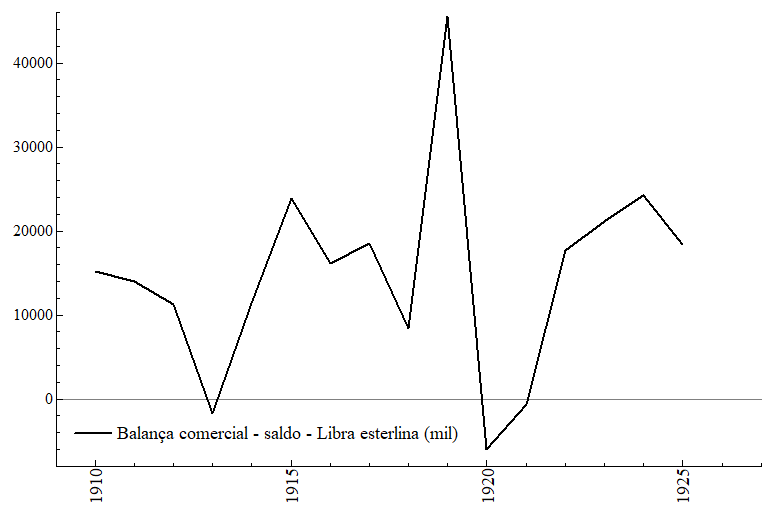
\includegraphics[width=1.0\textwidth]{i1d3.png}
    \end{figure}

O gráfico mostra uma clara reversão na balança comercial brasileira no biênio 1919/1920. Em 1919, observa-se um saldo comercial positivo significativo, seguido de uma queda acentuada para um déficit expressivo em 1920. Essa reversão pode ser explicada principalmente pela mudança no cenário externo, que influenciou fortemente a economia brasileira nesse período. Vamos analisar os fatores principais que explicam essa transformação:

\begin{itemize}
    \item \textbf{Superávit comercial de 1919:} O ano de 1919 marcou um dos momentos mais prósperos para a balança comercial brasileira, principalmente devido à alta demanda internacional por café, a principal commodity de exportação do país. Esse aumento da demanda foi impulsionado por dois fatores: a recuperação econômica dos países europeus após o fim da Primeira Guerra Mundial e a forte geada de 1918 que reduziu a oferta global de café, especialmente em São Paulo, onde a produção foi drasticamente afetada. Com uma oferta menor e uma demanda crescente, os preços do café subiram consideravelmente, resultando em um aumento expressivo nas receitas de exportação. Isso, por sua vez, gerou um superávit comercial substancial para o Brasil.
    
    \item \textbf{Mudanças globais em 1920:} O ano de 1920 trouxe uma reviravolta no cenário econômico global. As principais economias do mundo, particularmente os Estados Unidos e o Reino Unido, adotaram políticas monetárias restritivas com o objetivo de combater a inflação pós-guerra. Essas políticas resultaram em uma desaceleração econômica global, que teve um efeito negativo sobre o comércio internacional. A demanda por commodities, incluindo o café, caiu drasticamente, o que impactou diretamente as exportações brasileiras. A queda nos preços das commodities, em especial do café, foi um fator chave para o colapso do superávit comercial obtido no ano anterior.
    
    \item \textbf{Aumento das importações e crise cambial:} Paralelamente à queda nas exportações, o Brasil experimentou um aumento tardio nas importações em 1920. Com a retomada do crescimento econômico após o término da guerra, o país aumentou suas compras de bens de capital e produtos manufaturados, essenciais para o desenvolvimento de sua infraestrutura e indústria. Esse aumento nas importações, somado à queda nas exportações, criou um desequilíbrio na balança comercial. A pressão sobre a balança de pagamentos também levou a uma crise cambial, com a desvalorização do mil-réis. A desvalorização da moeda impactou ainda mais os custos das importações, ampliando o déficit comercial.
    
    \item \textbf{Consequências para a economia brasileira:} O déficit comercial de 1920 refletiu a vulnerabilidade da economia brasileira às flutuações do mercado internacional e à dependência de um número limitado de produtos de exportação, principalmente o café. A queda dos preços internacionais das commodities, combinada com o aumento das importações e a crise cambial, gerou uma crise econômica que impactou não apenas o comércio exterior, mas também a política fiscal e monetária interna. O governo foi forçado a adotar medidas de austeridade e buscar mecanismos de financiamento externo para lidar com o déficit e estabilizar a economia.
\end{itemize}

Em resumo, a reversão observada no gráfico, com um superávit em 1919 e um déficit em 1920, deve-se sobretudo a uma reversão no cenário externo, marcada pela queda da demanda global por commodities, políticas monetárias restritivas internacionais e o aumento das importações brasileiras. Essas condições externamente impostas tiveram um impacto profundo na economia do Brasil, refletindo sua vulnerabilidade às condições do mercado internacional e à sua forte dependência de exportações de produtos primários.

\subsection{\textbf{No gráfico a seguir, podemos notar uma grande depreciação da taxa de câmbio brasileira no início da década de 1920. Esse movimento cambial foi consequência exclusiva do cenário de grandes dificuldades econômicas derivadas da conjuntura global. Você concorda com essa avaliação? Explique.}}

\begin{figure}[H]
    \centering
    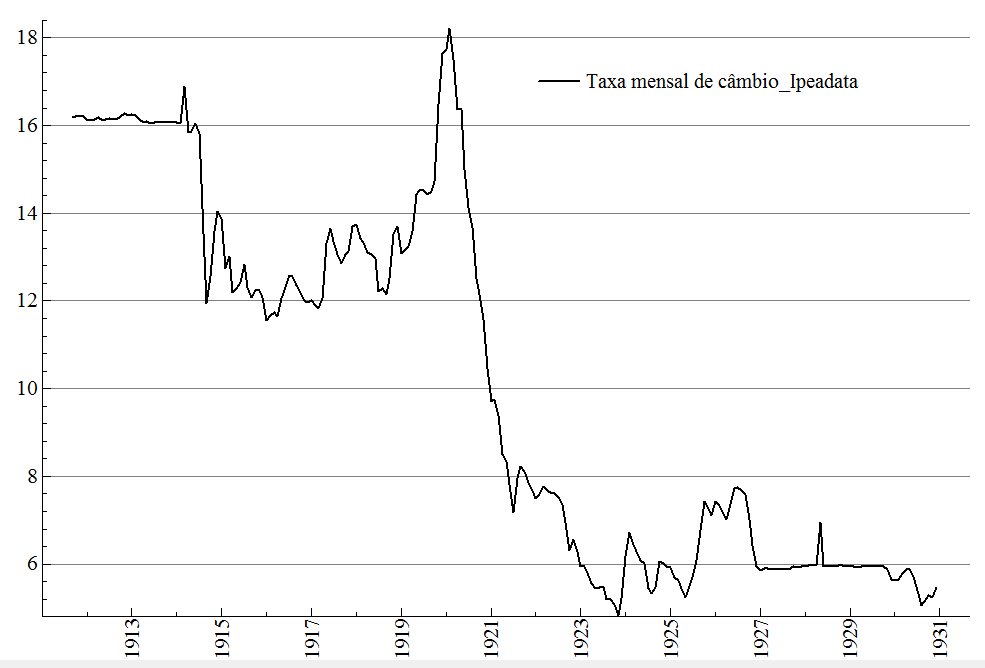
\includegraphics[width=1.0\textwidth]{i2d3.png}
    \end{figure}

\subsection{\textbf{No gráfico a seguir, podemos notar uma grande depreciação da taxa de câmbio brasileira no início da década de 1920. Esse movimento cambial foi consequência exclusiva do cenário de grandes dificuldades econômicas derivadas da conjuntura global. Você concorda com essa avaliação? Explique.}}

O gráfico apresenta uma depreciação acentuada da taxa de câmbio brasileira no início dos anos 1920. Esse movimento não foi causado exclusivamente por dificuldades econômicas internacionais, embora os fatores globais tenham desempenhado um papel importante. A seguir, detalharemos os principais fatores que contribuíram para essa desvalorização cambial, tanto no âmbito externo quanto no interno.

\begin{itemize}
    \item \textbf{Fatores externos:}
    O período pós-Primeira Guerra Mundial trouxe um cenário econômico internacional desafiador. As principais economias globais, como Estados Unidos e Reino Unido, estavam focadas em combater as pressões inflacionárias que surgiram devido aos altos gastos durante a guerra. Para isso, adotaram políticas monetárias restritivas, como o aumento das taxas de juros e a redução da oferta monetária. Essas medidas reduziram a liquidez internacional e dificultaram o comércio global. Para países exportadores de commodities, como o Brasil, essas políticas resultaram em uma queda na demanda por seus produtos no mercado internacional, especialmente o café, a principal exportação brasileira da época. 
    
    A queda dos preços das commodities no mercado internacional, como o café, agravou a situação. Em 1920, o Brasil sofreu uma queda abrupta nas receitas de exportação devido à combinação de uma redução global na demanda e uma queda nos preços. Com uma balança comercial deficitária, o país teve que recorrer a reservas cambiais para pagar suas importações, o que exerceu forte pressão sobre a taxa de câmbio, resultando na depreciação do mil-réis.
    
    \item \textbf{Fatores internos:}
    Embora o cenário internacional tenha sido desfavorável, os problemas internos do Brasil também desempenharam um papel fundamental na desvalorização cambial. A economia brasileira era fortemente dependente de suas exportações de café, o que deixava o país vulnerável a flutuações nos preços internacionais dessa commodity. Quando os preços do café caíram em 1920, as receitas do país diminuíram, agravando o desequilíbrio nas contas externas.
    
    Além disso, o Brasil enfrentava desafios fiscais e monetários significativos. Durante esse período, o governo brasileiro adotou políticas monetárias expansionistas para financiar o déficit público e sustentar a política de valorização do café, que consistia na compra de estoques excedentes de café para evitar a queda dos preços internacionais. Essa política exigia recursos financeiros significativos, levando o governo a emitir grandes quantidades de moeda. Essa emissão descontrolada de papel-moeda, sem o devido lastro em reservas cambiais, ampliou a base monetária e alimentou a inflação interna.
    
    \item \textbf{Crise cambial e de dívida pública:}
    A crise cambial de 1920-1921 foi amplificada pelo aumento da dívida pública, que crescia devido à necessidade de financiamento do setor cafeeiro e de obras públicas. Com uma economia fragilizada, o governo recorreu à emissão de notas inconversíveis para cobrir seus gastos. Esse aumento da base monetária, em um contexto de baixa entrada de divisas estrangeiras, resultou em uma depreciação adicional do mil-réis. A desvalorização da moeda intensificou a inflação, afetando os custos de importação e reduzindo o poder de compra da população.
    
    \item \textbf{Desafios na balança de pagamentos:}
    O déficit na balança de pagamentos também foi agravado pelo aumento das importações, já que o Brasil dependia de bens de capital e produtos manufaturados importados para seu desenvolvimento econômico. No entanto, a queda das exportações e o aumento das importações geraram um desequilíbrio comercial ainda maior. Com uma balança de pagamentos deficitária, o Brasil viu suas reservas cambiais diminuírem rapidamente, o que pressionou ainda mais o câmbio. A desvalorização do mil-réis foi inevitável, visto que a demanda por divisas estrangeiras superava a oferta disponível.
    
    \item \textbf{Política de austeridade e tentativas de estabilização:}
    Como resposta à crise cambial e à inflação crescente, o governo brasileiro tentou adotar medidas de austeridade fiscal, incluindo cortes nos gastos públicos e aumentos nas taxas de juros, para conter a inflação e estabilizar a moeda. No entanto, essas medidas foram insuficientes no curto prazo, uma vez que a economia brasileira ainda era muito vulnerável às flutuações no comércio internacional e à dependência de um número limitado de produtos de exportação, como o café. A recuperação econômica foi lenta e a desvalorização cambial continuou a ser um problema ao longo dos anos 1920.
\end{itemize}

Em conclusão, embora o cenário global tenha desempenhado um papel importante na depreciação da taxa de câmbio brasileira no início da década de 1920, essa desvalorização não foi causada exclusivamente por fatores externos. A política fiscal e monetária interna, caracterizada pela emissão descontrolada de moeda e pela alta dependência das exportações de café, foi igualmente responsável pelo movimento cambial. A combinação de pressões globais e desequilíbrios internos levou à desvalorização do mil-réis, demonstrando a vulnerabilidade da economia brasileira durante esse período.

\end{document}